

\documentclass[handout]{beamer}
\setbeamertemplate{caption}{\raggedright\insertcaption\par}
 
\usepackage[utf8]{inputenc}

\usetheme{Boadilla}
\usecolortheme{default}
\usepackage{dsfont}
\usepackage{multirow}

\setbeameroption{hide notes}







 
%Information to be included in the title page:
\title[Introduction to Causality] %optional
{Introduction to Causality}
 
%\subtitle{A short story }
 
%\author[Wang, Webb, Rainforth] % (optional, for multiple authors)
%{Benjie Wang, Stefan Webb, Tom Rainforth}

 
 
\date[04/02/2019] % (optional)
{}
 


\AtBeginSection[]
{
  \begin{frame}
    \frametitle{Table of Contents}
    \tableofcontents[currentsection]
  \end{frame}
}


 
\begin{document}
 
\frame{\titlepage}

\note[]{
  This lecture will be light on maths/methods
  About thinking conceptually about causality
}

 
\section{Introduction}
\begin{frame}
\frametitle{Motivation}
\pause
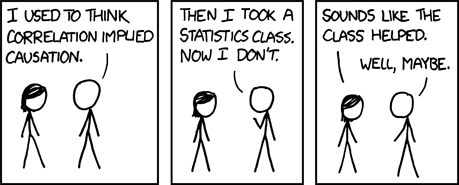
\includegraphics[scale=0.8]{figures/correlation.png}
\note[]{
We've all heard "C does not imply C". But it's not just that. Instead of defining what causality isn't, can we define what it is? And then can we use causality to help machines reason about the world?
}
\end{frame}
\begin{frame}
\frametitle{Motivation}

Why is this such a key question? \pause
\medskip

\textbf{Stability:} Causal relationships are robust to external change. \pause

\medskip
How does the human brain think about causality?
\bigskip

\note[]{
Why is causality so fundamental in an understanding of the world?
Whole problem of machine learning: distributional shift
Not so interested in physical/QM basis of causality, but how humans infer causal relationships and reason about these to further their goals.
Match or oxygen?
How can an elephant be in a china shop? 
}


\includegraphics[width=0.303\textwidth]{figures/candles.jpg}%
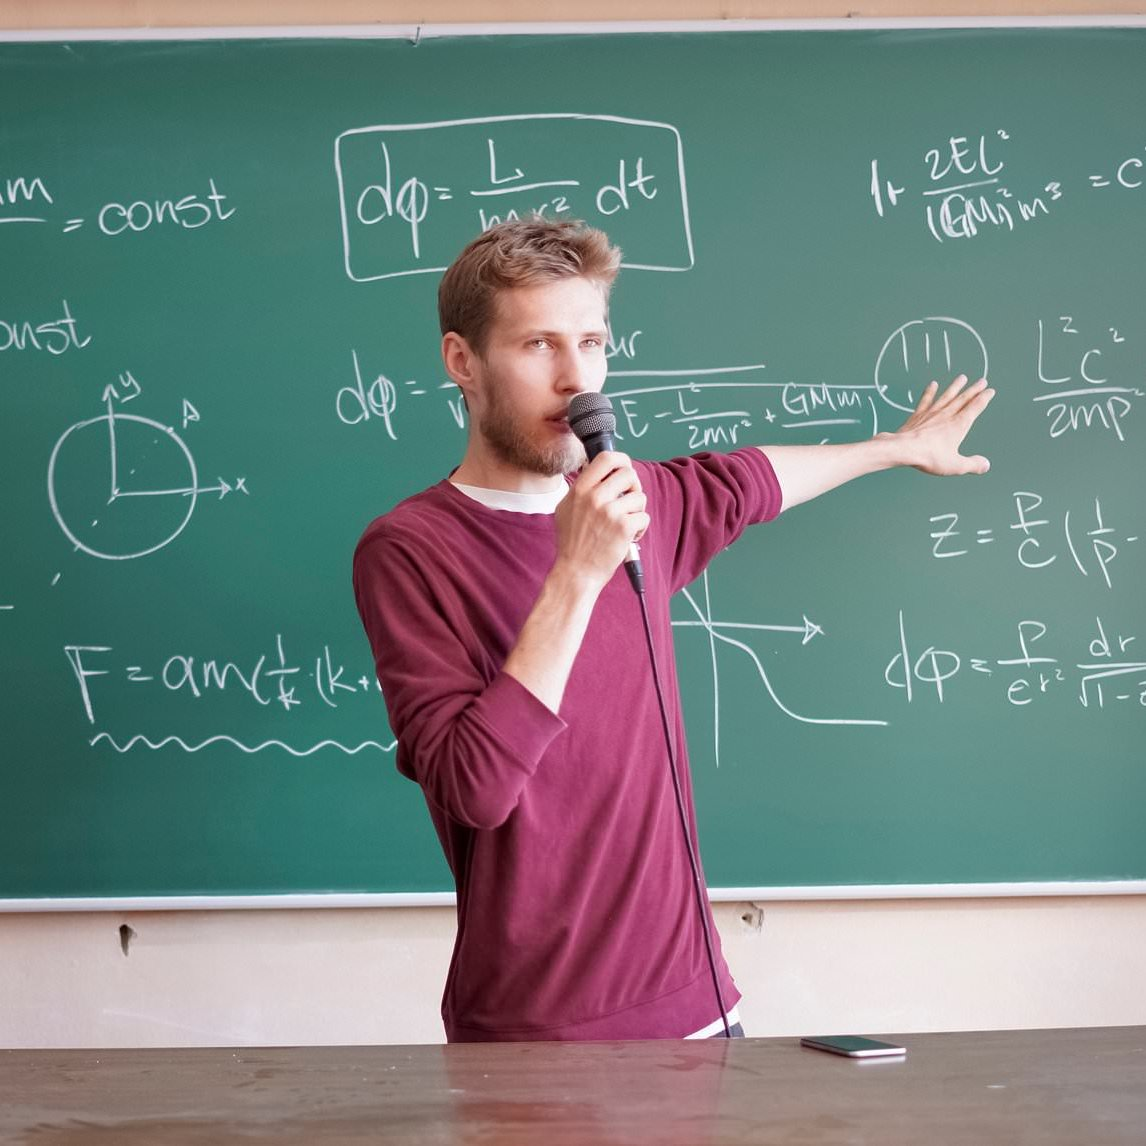
\includegraphics[width=0.303\textwidth]{figures/teacher.jpg}
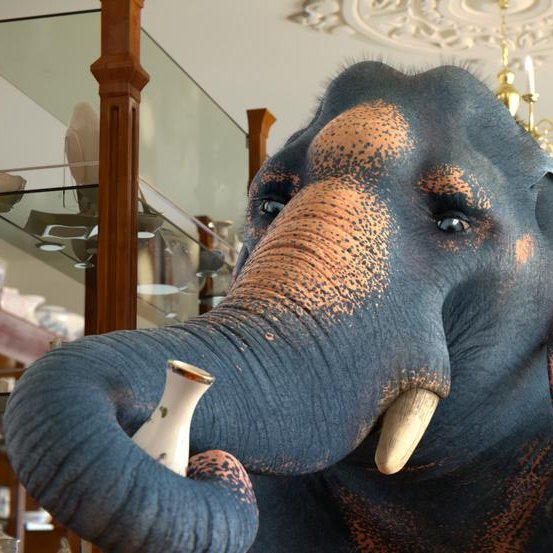
\includegraphics[width=0.3\textwidth]{figures/elephant.jpg}
         
\end{frame}

\begin{frame}
\frametitle{Motivation}

\begin{center}
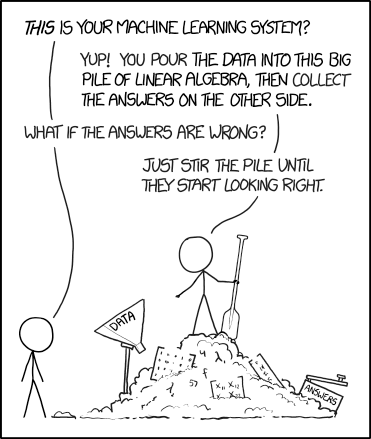
\includegraphics[scale=0.45]{figures/xkcd_data.png}
\end{center}
         
\end{frame}

\begin{frame}
\frametitle{Example: Distribution shift}
Suppose we are trying to classify images $\textbf{x}$ of cats or dogs (label $\textbf{y}$), and we learn a NN $p(\textbf{y}|\textbf{x})$ for this task.

\pause
\bigskip
Now let's assume we go to a different "environment". What might have changed?
\pause
\begin{itemize}
	\item $p(y)$: Maybe there are more cats in dogs in some countries...
	\pause
	\item $p(x|y)$: Maybe we see different breeds of dog more often. Or we capture the image in different conditions, e.g. day/night
	\pause
	\item $p(y|x)$: ??
\end{itemize}

\note[]{
	
}
\end{frame}


\begin{frame}
\frametitle{Questions} \pause
\begin{itemize}
\item What does "A causes/caused B" mean? \pause
\item How can we infer causal relationships? \pause
\item How can we represent and use causal information? \pause
\end{itemize}
\note[]{
Will talk about the first two together primarily in this lecture. They are closely related and often conflated (positing a method for inferring causality and a posteriori using this as the definition for causality)
But third is perhaps most important and we will go into detail next lecture
}
\end{frame}


\begin{frame}
\frametitle{Defining causality: Things to consider}
\begin{itemize}
	\item \textbf{Type/token level}: Suppose medicine A causes most patients to recover (B), but also had no effect or killed a small minority of patients ($\neg$B). \pause
	\item \textbf{Necessary/Sufficient cause}: Do we assert there is no alternative cause for B, or that A alone can cause B? 
\end{itemize}
\note[]{
We might say different things depending on the context we're talking about.
Both can make sense 
}
\end{frame}

\begin{frame}
\frametitle{Characterizing causality: a first attempt}
\begin{table}[]
\begin{tabular}{|p{3.7 cm}|p{5cm}|p{2cm}|}
\hline
\textbf{Name}                   & \textbf{Language}                                      & \textbf{N/S?} \\ \hline
Association                     & "A makes B more likely"                                &               \\ \hline
Temporal Precedence             & "A comes before B"                                     & N             \\ \hline
Counterfactuals                 & "If A had been different, B might have been different" & S             \\ \hline
Physical Mechanism/ Direct Cause & "There is some mechanism through which A influences B" & N, S          \\ \hline
\end{tabular}
\end{table}
\note[]{
Focus on human thought
N/S means different thing here compared to previous slide
DAG examples - if familiar with BNs forget, if not, great, read it as a non-trained person would
}

\note[]{
How do we say, yes X caused Y?
Giving some intuition - no conclusive answers here
}
\end{frame}


\section{Approaches to defining causality}
\begin{frame}
\frametitle{Probabilistic Causality}
Long line of attempts in social sciences, economics and statistics.
\pause
\begin{itemize}
	\item Granger causality
	\pause
	\item Suppes (1970): "Probability raising" and "screening off using temporal precedence"
	\pause
	\item Eells (1991): Contexts, splitting up type/token-level causality
\end{itemize}
\pause
Usually assumes knowledge of \textbf{temporal precedence}
\end{frame}

\begin{frame}
\frametitle{Generic framework for probabilistic causality}
C is "causally relevant" for E if:
\pause
\begin{itemize}
	\item C precedes E temporally
	\pause
	\item $P(E|C) > P(E)$, i.e. "probability raising"
	\pause
	\item No common cause S of C and E (preceding both temporally) - \textit{Reichenbach's common cause principle}
\end{itemize}
\pause
The third is where probabilistic accounts of causality differ: some rely on "background contexts", some on enumerating possible causes, etc.
\note[]{
	But this leads to circularity; unclear how to define an appropriate background context without causal knowledge
}
\end{frame}

\begin{frame}
\frametitle{Pros and cons}
\begin{itemize}
\pause
\item Fairly easy to come up with heuristics (and many exist) for using association and temporal information
\pause
\item Can be of great practical utility in assisting humans in identifying/checking \textbf{potential} causes
\pause
\end{itemize}

but ....
\pause
\begin{itemize}
\item No model-based extension: cannot perform complex queries and reasoning
\pause
\item Not reliable: all heuristics will misidentify causes sometimes
\pause
\item Heuristics implicitly code in assumptions
\pause
\item Reliance on temporal information to break symmetry; this precludes application to many problems
\pause
\item Struggles to deal with token-level causality
\end{itemize}

\end{frame}

\begin{frame}
\frametitle{Counterfactual causality}

A \textbf{counterfactual statement} is one which expresses information about what \textit{did not happen}; i.e. a hypothetical. For example, "if $c$ happened, $e$ would have happened". \pause
\medskip

Lewis' (1973) counterfactual theory defined this statement using the notion of "possible worlds". Either: \pause
\begin{itemize}
	\item There are no possible $c$-worlds;
	\pause
	\item There exists an $c$-world where $e$ holds, which is closer to the actual world than any $c$-world in which $e$ does not hold
	\pause
\end{itemize}

Then, Lewis defines $e$ to be \textbf{causally dependent} on $c$ if:
\pause
\begin{itemize}
	\item "If $c$ was true, $e$ would be true"
	\pause
	\item "If $c$ was not true, then $e$ would not be true"
\end{itemize}


\note[]{

Lewis proposes "closest world in which A is true". We shall see the interpretation of potential outcomes and pearl in future
}
\end{frame}

\begin{frame}
\frametitle{Pros and Cons}
\begin{itemize}
	\item Axiomatic framework available which explicitly codes in assumptions;
	\item Can be extended compositionally with the idea of a "causal chain";
	\item Explicitly works on the unit/token level
\end{itemize}

but...

\begin{itemize}
	\item No obvious way to define "closest world", without invoking causality in a circular manner;
	\item Original formulation not probabilistic;
\end{itemize}

\end{frame}
\section{Queries and Models}

\begin{frame}
\frametitle{Why do we need a model?}
Definitions of causality are good ... but we want to be able to reason/answer causal queries. 
\pause

Here are some natural language queries:
\pause
\begin{itemize}
	\item Does A cause B?
	\pause
	\item What caused B?
	\pause
	\item Did A cause B?
	\pause
	\item What distribution over B (lung cancer) does forcing someone to smoke (A = 1) cause compared to the general population?
	\pause
\end{itemize}

\textbf{Associations}: Given A is 1, what is the distribution on B?
\pause

\textbf{Interventions}: If we fix A to be 1 ($do(A=1)$), then what is the distribution on B?
\pause

\textbf{Counterfactuals}: In a specific situation where we observed $C=c$, if we fix A to be 1, then what is the distribution on B?
\pause
\end{frame}

\begin{frame}

\frametitle{Modelling}

We need a \textbf{model}: a representation of reality which allows us to assign truth values to relevant statements through some computational procedure.
\pause
e.g. 
\begin{itemize}
	\item \textbf{Truth tables} are a model for evaluating Boolean expressions
	\item \textbf{Joint probability distributions} are a model for evaluating conditional probabilities, conditional independences
\end{itemize}
\pause
A \textbf{causal} model needs to encode the truth values of causal statements, e.g. counterfactuals. Probability distributions over variables are not sufficient for a causal model: need additional \textbf{assumptions}.
\pause
\bigskip
Two main frameworks: \textbf{Potential Outcomes (PO)} and \textbf{Structural Causal Models (SCM)}.

\note[]{
Use whiteboard to write up truth tables/joint probability distributions
Causal statements represent information about external changes to the environment.
Probability distributions are not sufficient: they cannot generalize to alternate realities.
Frameworks are equivalent. Any assumption in one can be translated to another. However their different representational formats make them more amenable to some tasks.
}

\end{frame}

\begin{frame}
\frametitle{Counterfactual Notation}
Idea: Define counterfactuals explicitly as counterfactual \textbf{random variables} on a probability space $(U, \mathcal{F}, p)$, even though we can never observe them.

\medskip
Here $u \in U$ represents "all relevant randomness".

\pause
\bigskip
$Y_x$ is the counterfactual random variable "the value of Y, had X been x". That is, we set/intervene $X$ to be $x$. The randomness is over $u$.

\pause
\bigskip
We can then define queries such as:
\begin{itemize} 
    \item $\pmb{p(Y_{x} = y)}$: "probability that $Y$ is $y$ if we set $X$ to be $x$"
    \pause
	\item $\pmb{p(Y_{x'} = y' | X = x, Y = y)}$: "probability that $Y$ would have been $y'$ if $X$ were $x'$, given that we actually observed $X=x$ and $Y=y$"
	\pause
	\item $\pmb{p(Y_x = y, Y_{x'} = y')}$
\end{itemize}




\note[]{
  Draw table on board with missing data
  Think of $u$ as the individual.
  First example is "intervention", second is "counterfactual".
}
\end{frame}

\begin{frame}
\frametitle{Rubin Causal Model (Potential Outcomes): A statistical/algebraic approach to counterfactals}

In PO framework, we define counterfactual variables $Y_x$ as primitives. Thus, it is simple to answer causal queries of the type we have described.
\pause

\bigskip
Causal knowledge is represented as knowledge of about the probability distribution over counterfactual variables, e.g. $p(X, Y_{z=0}, Y_{z=1})$ where $Z$ is a binary treatment.
\pause

\bigskip
However, it can be very difficult to specify such as distribution, especially when there are many variables involved; might need to work with conditional independences and algebraic manipulation.

\end{frame}

\begin{frame}
\frametitle{Pearl's SCMs (Structural Causal Models): A structural approach to counterfactuals}

Model represented by a graph and set of \textbf{structural equations}:
\pause

$$v_i = f_i(\text{pa}_i, u_i)$$
\pause

where $v_i$ are variables, $pa_i$ represent the parents of $v_i$ in the graph, and $u_i$ are "background variables". We make the model probabilistic by additionally including a distribution $p(u)$.
\pause

\bigskip
This representation is sufficient to answer all of the causal queries we have previously mentioned.
\pause

\note[]{
 Graph/explanation on board
}


\end{frame}

\begin{frame}
\frametitle{Takeaways}
\begin{itemize}
	\item Causal relationships are useful because they are \textbf{stable};
	\item All causal questions can be expressed in terms of counterfactuals;
	\item In order for a machine to reason about causal queries, they need a \textbf{causal model};
	\item A \textbf{causal model} requires assumptions which cannot always be inferred from observational data
	\item Pearl's SCMs are widely used in causal inference and machine learning
\end{itemize}
\end{frame}

%Potential outcomes:
%\begin{itemize}
%	\item Treat counterfactuals as primitives
%	\item Assumptions/knowledge expressed as conditional independences
%\end{itemize}

%Structural causal models:
%\begin{itemize}
%	\item Treat direct causation as primitive
%	\item Assumptions/knowledge expressed as graphical structure and using %equations
%\end{itemize}

\end{document}

